\documentclass[12pt]{article}
%Gumm{\color{blue}i}|065|=)
\usepackage{amsmath, amsfonts, amssymb}
\usepackage[margin=0.5in]{geometry}
\usepackage{xcolor}
\usepackage{graphicx}
\usepackage{amsmath}

\newcommand{\off}[1]{}
\DeclareMathSizes{20}{30}{20}{18}
\usepackage{tikz}


\title{Scratchwork: Class Field Theory}
\date{}
\begin{document}

\sffamily

\maketitle

\noindent One common mistake is to say the ring of integers of $K =  \mathbb{Q}(\sqrt{-5})$ is $\mathbb{Z}[\sqrt{-5}]$.  In fact it's $\mathbb{Z}[\frac{1+\sqrt{-5}}{2}]$. This example is important because it's the first time we observe the failure of unique factorization in ``integers":
$$2 \times 3 = (1 + \sqrt{-5}) \times (1 - \sqrt{-5}) $$
Despite being quite well-known, I feel this is the kind of result that needs to be checked very carefully.  Number Theory in particular, is known to re-arrange obvious facts in shocking ways:
$$ \left( \frac{1 + \sqrt{-5}}{2} \right)^2 = \frac{1}{4} + \sqrt{-5} - \frac{5}{4} 
= 2 \times \left( \frac{1 + \sqrt{-5}}{2} \right) - 2 \times 1$$
What's so special about the $\sqrt{-5}$ that we obtain a number field with class number $h(K)=2$ ? \\ \\
\textbf{Ex} Factor the numbers $1 \leq n \leq 100$ in each of the two orders, $\mathcal{O}_1 = \mathbb{Z}\left[ \frac{1 + \sqrt{-5}}{2}\right]$ and $\mathcal{O}_2 = \mathbb{Z}[\sqrt{-5}]$. \\ \\
\textbf{Ex} Show that the ring of integers of $\mathbb{Q}(\sqrt{-5})$ is $\mathbb{Z}\left[ \frac{1 + \sqrt{-5}}{2}\right]$. \\ \\
Let's try to draw the ideal $(2)$. \\ \\
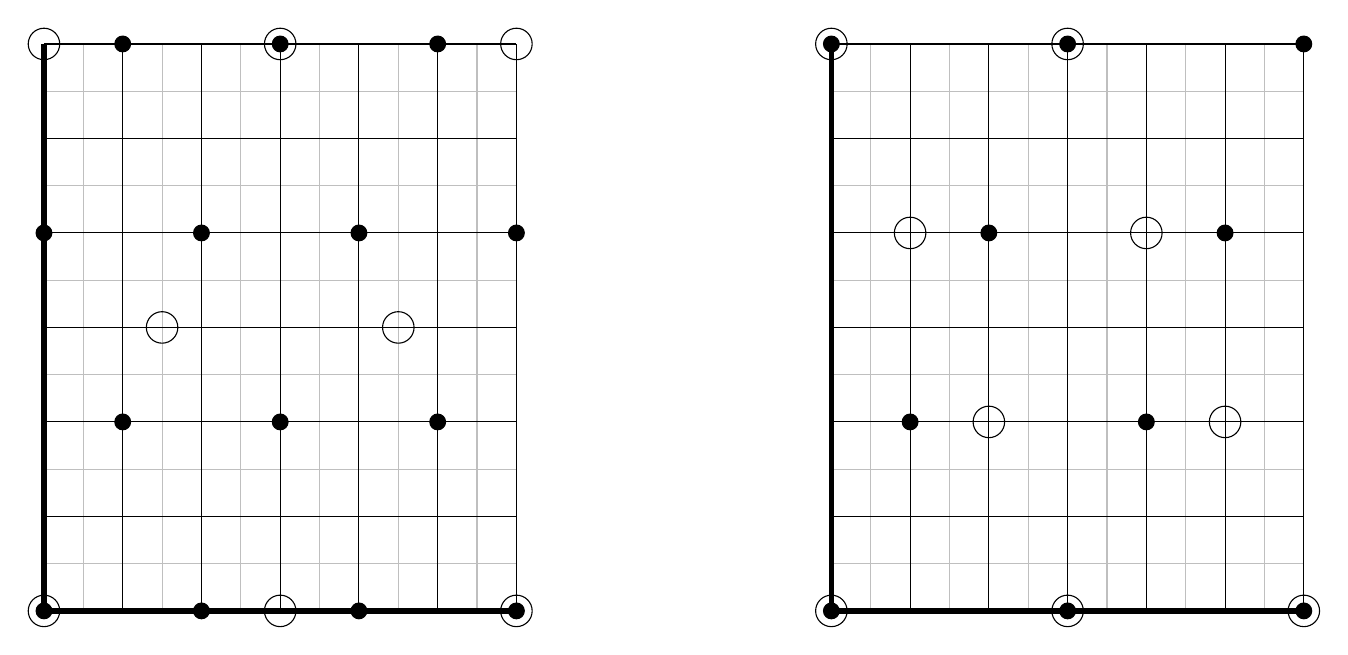
\begin{tikzpicture}[scale=1]

\begin{scope}


\foreach \a in {0,0.5,...,6}{
	\draw[black!25!white] (\a, 0)--(\a,6*1.2);
}

\foreach \a in {0,0.5,...,6}{
	\draw[black!25!white] (0,\a*1.2)--(6,\a*1.2);
}

\foreach \a in {0,...,6}{
	\draw (\a, 0)--(\a,6*1.2);
}

\foreach \a in {0,...,6}{
	\draw (0,\a*1.2)--(6,\a*1.2);
}

\draw[line width=2] (0,0)--(0,6*1.2);
\draw[line width=2] (0,0)--(6,0);

\draw[fill=black] (0,0*1.2) circle (0.1);
\draw[fill=black] (2,0*1.2) circle (0.1);
\draw[fill=black] (4,0*1.2) circle (0.1);
\draw[fill=black] (6,0*1.2) circle (0.1);

\draw[fill=black] (1,2*1.2) circle (0.1);
\draw[fill=black] (3,2*1.2) circle (0.1);
\draw[fill=black] (5,2*1.2) circle (0.1);

\draw[fill=black] (0,4*1.2) circle (0.1);
\draw[fill=black] (2,4*1.2) circle (0.1);
\draw[fill=black] (4,4*1.2) circle (0.1);
\draw[fill=black] (6,4*1.2) circle (0.1);

\draw[fill=black] (1,6*1.2) circle (0.1);
\draw[fill=black] (3,6*1.2) circle (0.1);
\draw[fill=black] (5,6*1.2) circle (0.1);

\draw (0,0*1.2) circle (0.2);
\draw (3,0*1.2) circle (0.2);
\draw (6,0*1.2) circle (0.2);

\draw (1.5, 3*1.2) circle (0.2);
\draw (4.5, 3*1.2) circle (0.2);

\draw (0,6*1.2) circle (0.2);
\draw (3,6*1.2) circle (0.2);
\draw (6,6*1.2) circle (0.2);

\end{scope}

\begin{scope}[xshift=10cm]


\foreach \a in {0,0.5,...,6}{
	\draw[black!25!white] (\a, 0)--(\a,6*1.2);
}

\foreach \a in {0,0.5,...,6}{
	\draw[black!25!white] (0,\a*1.2)--(6,\a*1.2);
}

\foreach \a in {0,...,6}{
	\draw (\a, 0)--(\a,6*1.2);
}

\foreach \a in {0,...,6}{
	\draw (0,\a*1.2)--(6,\a*1.2);
}

\draw[line width=2] (0,0)--(0,6*1.2);
\draw[line width=2] (0,0)--(6,0);

\draw[fill=black] (0,0*1.2) circle (0.1);
\draw[fill=black] (1,2*1.2) circle (0.1);
\draw[fill=black] (2,4*1.2) circle (0.1);
\draw[fill=black] (3,6*1.2) circle (0.1);

%\draw[fill=black] (-2,2*1.2) circle (0.1);
%\draw[fill=black] (-1,4*1.2) circle (0.1);
\draw[fill=black] ( 0,6*1.2) circle (0.1);

\draw[fill=black] (3,0*1.2) circle (0.1);
\draw[fill=black] (4,2*1.2) circle (0.1);
\draw[fill=black] (5,4*1.2) circle (0.1);
\draw[fill=black] (6,6*1.2) circle (0.1);

\draw[fill=black] (6,0*1.2) circle (0.1);

\draw (0,0) circle (0.2);
\draw (3,0) circle (0.2);
\draw (6,0) circle (0.2);

\draw (2,2*1.2) circle (0.2);
\draw (1,4*1.2) circle (0.2);
\draw (0,6*1.2) circle (0.2);

\draw (5,2*1.2) circle (0.2);
\draw (4,4*1.2) circle (0.2);
\draw (3,6*1.2) circle (0.2);



\end{scope}

\end{tikzpicture} \\ \\
Also $(3)$ and on the right hand side $(1 + \sqrt{-5})$ and $(1-\sqrt{-5})$. \\ \\
That was much harder than it should have been.  Btw, do you believe this?  This is what happens when we use a calculator and get the correct answer.  And it's perfectly good.

\begin{verbatim}
>>> 5**0.5/2
1.118033988749895
\end{verbatim}

\vfill
\begin{thebibliography}{}

\item Henri Cohen \textbf{Computational Number Theory in Relation with L-Functions} \texttt{arXiv:1809.10904}

\end{thebibliography}

\end{document}